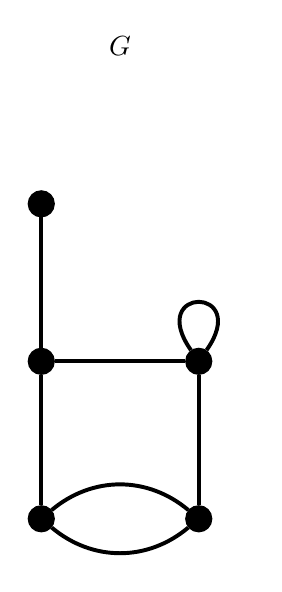
\begin{tikzpicture}
    \begin{scope}[xshift=0cm, yshift=0cm]
        \node (G) at (1, 6) {$G$};

        \node[circle, draw, fill=black, minimum size=0.01mm] (1) at (0, 4) {};
        \node[circle, draw, fill=black, minimum size=0.01mm] (2) at (0, 2) {};
        \node[circle, draw, fill=black, minimum size=0.01mm] (3) at (0, 0) {};
        \node[circle, draw, fill=black, minimum size=0.01mm] (4) at (2, 2) {};
        \node[circle, draw, fill=black, minimum size=0.01mm] (5) at (2, 0) {};

        % Draw the edges between nodes
        \draw[line width=0.5mm] (1) -- (2);
        \draw[line width=0.5mm] (2) -- (3);
        \draw[line width=0.5mm] (2) -- (4);
        \draw[line width=0.5mm] (4) -- (5);
        \draw[line width=0.5mm] (3) to[bend left=40] (5);
        \draw[line width=0.5mm] (3) to[bend right=40] (5);
        \draw[line width=0.5mm] (4) to[in=125,out=55,loop, min distance=1cm] (4);
    \end{scope}
\end{tikzpicture}
